\documentclass[conference]{IEEEtran}
\IEEEoverridecommandlockouts
\usepackage{cite}
\usepackage{amsmath,amssymb,amsfonts}
\usepackage{graphicx}
\usepackage{textcomp}
\usepackage{xcolor}
\usepackage{booktabs}
\usepackage{bm}
\usepackage[hidelinks]{hyperref}
\usepackage{url}
\newcommand{\Lles}{\mathcal{L}_{\mathrm{les}}}
\newcommand{\Lart}{\mathcal{L}_{\mathrm{art}}}

\begin{document}

\title{Lesion-Anchored Prototypes: Reducing Artifact Shortcuts in Interpretable Melanoma Classification\thanks{*Corresponding author: Fatemeh Ziaeetabar (fziaeetabar@ut.ac.ir).}}

\author{\IEEEauthorblockN{Yousef Azizi Movahed}
\IEEEauthorblockA{\textit{Dept. of Computer Science, School of Mathematics,}\\
\textit{Statistics, and Computer Science, College of Science}\\
\textit{University of Tehran}, Tehran, Iran\\
azizi.movahed@ut.ac.ir}
\and
\IEEEauthorblockN{Fatemeh Ziaeetabar*}
\IEEEauthorblockA{\textit{Dept. of Computer Science, School of Mathematics,}\\
\textit{Statistics, and Computer Science, College of Science}\\
\textit{University of Tehran}, Tehran, Iran\\
fziaeetabar@ut.ac.ir}
}

\maketitle

\begin{abstract}
Melanoma classifiers often pick up acquisition artifacts such as dark corners, rulers and ink. In a prototype-based network the consequence is worse than a biased prediction: the explanation itself (``this part looks like that prototype'') can point at the artifact. We first measure the problem on ISIC~2019: dark corners and bright specular structures are significantly associated with melanoma even after stratifying by acquisition source (Mantel--Haenszel odds ratios 1.56 and 1.75), and a black-box DenseNet-121 places its class-activation maps on artifacts 1.5 times more often than their area would predict. Existing remedies either need expert annotation of relevant regions or act on accuracy alone, and none controls \emph{which} training patches a prototype may become. We propose lesion-anchored prototype learning with two components: a lesion-attraction objective on the spatial attention of each prototype, and a projection step that only admits artifact-free lesion patches, so that every prototype is lesion tissue by construction. Both are supervised by automatically generated masks; we document their provenance, validate them (Dice 0.945 on held-out expert masks, 0.918 on the external PH2 set), show that the classifier needs no mask at inference, and audit the split for leakage. With an identical backbone, split and training budget (three seeds), the approach raises the test AUC of ProtoPNet from 0.825 to 0.865 (fine-annotation baseline: 0.844), places all prototypes on lesion tissue, and lowers the share of the explanation hot region on artifacts from 6.6\% to 4.8\%. In counterfactual tests that insert or remove artifacts while every lesion pixel stays unchanged, it roughly halves the decision-flip rate of ProtoPNet for dark corners and rulers (e.g., 10.9\%$\rightarrow$5.2\%) and keeps its explanations stable (Spearman 0.92 vs.\ 0.68). An additional artifact-suppression term turned out to be unnecessary, which we report as a negative result. Code, executed notebooks and logs: \url{https://github.com/YousefAMovahed/lesion-anchored-prototypes}.
\end{abstract}

\begin{IEEEkeywords}
explainable AI, prototypical part networks, shortcut learning, dermoscopy artifacts, melanoma, counterfactual evaluation
\end{IEEEkeywords}

\section{Introduction}
Convolutional networks can classify skin lesions as accurately as dermatologists~\cite{esteva2017}, but they also learn \emph{shortcuts}~\cite{geirhos2020}, i.e.\ features that happen to correlate with the label in the training data without being related to the disease. Dermoscopy offers several documented cases. Surgical skin markings raise the melanoma probability of a deep classifier~\cite{winkler2019}, and models still perform far above chance when the lesion is removed from the image~\cite{bissoto2019,bissoto2020}. Dark corners, rulers, gel bubbles and ink are frequent in public archives and unevenly distributed across acquisition sites~\cite{bissoto2022,yan2023}.

For clinical use, Rudin~\cite{rudin2019} argues for models that are interpretable by design rather than explained after the fact. The prototypical part network (ProtoPNet)~\cite{chen2019} compares image patches with learned prototypes, each projected onto a real training patch, so that a decision reads ``this part looks like that part''. ProtoPNet does not, however, stop a prototype from being a piece of a ruler or of a black corner. In that case the shortcut survives and is in addition presented to the user as a reasonable explanation~\cite{hoffmann2021}. \textbf{Research gap.} Prior work leaves three things open (Table~\ref{tab:gap}). (i) Debiasing methods for dermoscopy~\cite{bissoto2022,yan2023,bevan2022} improve accuracy under artifact shift, but their models are black boxes, so nobody can see whether a decision rests on the lesion. (ii) Explanation-supervision methods~\cite{ross2017,rieger2020,barnett2021} do constrain where a model looks, but they need pixel-level annotation from experts, and for prototype networks they only shape the activation maps; the \emph{push} step, which decides which training patch a prototype finally \emph{is}, stays unconstrained, so a prototype can still be projected onto a ruler or a black corner. Human-in-the-loop debugging~\cite{bontempelli2023} removes such prototypes only after a user has found them. (iii) Explanations of prototype networks are rarely tested by intervening on the artifacts themselves; accuracy and qualitative heatmaps are the usual evidence.

\textbf{Contributions.} This paper fills these gaps with the following contributions.
\begin{itemize}
\item \textbf{Lesion-anchored prototype learning without manual annotation.} A lesion-attraction objective acts on the spatial attention of every prototype and pulls it towards lesion tissue. It is supervised only by automatically generated masks, with no expert annotation, and it is the component responsible for the accuracy gain (+4.0 AUC points over ProtoPNet).
\item \textbf{Lesion-constrained projection.} We restrict the push step to artifact-free lesion patches. Every prototype is then lesion tissue \emph{by construction}, a guarantee that loss-based methods cannot give. The ablation shows that this step leaves the accuracy unchanged but halves how much of the explanation an inserted artifact can capture.
\item \textbf{A counterfactual test of decisions \emph{and} explanations.} Four artifact types are inserted, and real hair and ruler marks are removed, while every lesion pixel stays bit-identical; an inpainting-only null control separates the effect of the artifact from that of the editing.
\item \textbf{A leakage-controlled and mask-audited evaluation.} We group near-duplicates in addition to lesion identifiers, document and validate the provenance of every mask, show that the classifier needs no mask at test time, compare eight configurations with the same backbone over three seeds, and test on three external sets.
\end{itemize}
An artifact-suppression loss that we also explored did not add any measurable benefit; we keep it in the ablation and discuss it as a negative result rather than as a contribution.

\section{Related Work}
\textbf{Artifacts and shortcuts in dermoscopy.} Bissoto \emph{et al.} showed that ISIC models perform well even when the lesion is occluded~\cite{bissoto2019}, annotated seven artifact types, found that simple debiasing does not remove the bias~\cite{bissoto2020}, and later used artifact annotations to build domain-generalization benchmarks~\cite{bissoto2022}. Winkler \emph{et al.}~\cite{winkler2019} reported that skin markings raise the melanoma score of a commercial-grade classifier. EPVT~\cite{yan2023} treats artifact groups as domains and learns domain prompts for a vision transformer, and Bevan and Atapour-Abarghouei~\cite{bevan2022} remove artifact information from the representation by adversarial unlearning. These methods measure success by accuracy under shift; the resulting models are not interpretable, and they need image-level artifact labels.

\textbf{Prototype-based interpretability.} ProtoPNet~\cite{chen2019} classifies by similarity to class-specific prototypes that are projected onto real training patches, which makes its reasoning inspectable~\cite{rudin2019}. Hoffmann \emph{et al.}~\cite{hoffmann2021} showed that the visual similarity suggested by such prototypes can be misleading, which motivates testing explanations rather than taking them at face value~\cite{adebayo2018}.

\textbf{Explanation supervision.} Right-for-the-right-reasons (RRR)~\cite{ross2017} penalizes input gradients inside annotated irrelevant regions, and CDEP~\cite{rieger2020} penalizes contextual-decomposition importance, demonstrated on ISIC images with colored patches. Closest to us, IAIA-BL~\cite{barnett2021} adds a fine-annotation loss to a prototype network that penalizes prototype activation outside regions marked by radiologists, and ProtoPDebug~\cite{bontempelli2023} lets a user mark confounded prototypes that are then forgotten. All of them need human input, either pixel-level masks or interactive feedback. More importantly, none of them constrains the projection step, which decides what a prototype finally is.

\begin{table}[t]
\caption{Positioning against related work. Annot.: human input required; Interp.: interpretable by design; Where: constrains where the explanation looks; Prov.: constrains which training patches prototypes become; CF: explanations tested under artifact interventions.}
\label{tab:gap}
\centering
\setlength{\tabcolsep}{2.6pt}
\begin{tabular}{lccccc}
\toprule
Method & Annot. & Interp. & Where & Prov. & CF \\
\midrule
EPVT~\cite{yan2023}, unlearning~\cite{bevan2022} & image labels & -- & -- & -- & -- \\
RRR~\cite{ross2017}, CDEP~\cite{rieger2020} & pixel masks & -- & \checkmark & -- & -- \\
ProtoPNet~\cite{chen2019} & none & \checkmark & -- & -- & -- \\
IAIA-BL~\cite{barnett2021} & expert masks & \checkmark & \checkmark & -- & -- \\
ProtoPDebug~\cite{bontempelli2023} & user feedback & \checkmark & -- & post hoc & -- \\
\textbf{Ours} & \textbf{none (auto.)} & \checkmark & \checkmark & \checkmark & \checkmark \\
\bottomrule
\end{tabular}
\end{table}

\section{Method}
\subsection{Prototypical part network}
We build on a DenseNet-121 backbone~\cite{huang2017}. Two $1\times1$ convolutions with a final sigmoid turn its output into a latent map $z\in[0,1]^{H\times W\times D}$, here with $H=W=7$ and $D=128$. The network keeps $m=20$ prototypes $p_j\in\mathbb{R}^D$, ten for each class, and $c(j)$ denotes the class of prototype $j$. For every cell we compute the distance $d_j(h,w)=\lVert z_{hw}-p_j\rVert_2^2$ and convert it into a similarity $s_j(h,w)=\log\frac{d_j(h,w)+1}{d_j(h,w)+\epsilon}$ with $\epsilon=10^{-4}$. A prototype is as active as its best-matching cell, $a_j=\max_{h,w}s_j(h,w)$, and the logits are $\mathbf{W}\bm{a}$. Training minimizes
\begin{equation}
\mathcal{L}=\mathcal{L}_{\mathrm{CE}}+\lambda_c\mathcal{L}_{\mathrm{clst}}-\lambda_s\mathcal{L}_{\mathrm{sep}}+\lambda_l\Lles+\lambda_a\Lart ,
\label{eq:loss}
\end{equation}
in which $\mathcal{L}_{\mathrm{CE}}$ is a class-weighted cross-entropy, while the cluster and separation costs measure the distance to the closest prototype of the own and of the other class~\cite{chen2019}. We keep the original weights $\lambda_c=0.8$ and $\lambda_s=0.08$. The proposed approach consists of the lesion-attraction term $\Lles$ ($\lambda_l=1$) and the constrained projection of Section~\ref{sec:push}; the artifact-suppression term $\Lart$ ($\lambda_a=1$ in our main runs, $\lambda_a=0$ in the ablation) is examined separately in Section~\ref{sec:lart}. All three use lesion and artifact masks whose construction and validation are described in Section~\ref{sec:masks}.

\subsection{Lesion attraction (core component)}
During training the masks undergo the same geometric augmentation as the image. Average pooling to the $7\times7$ grid then gives, for each cell, the fraction covered by lesion, $M^L(h,w)$, and by artifacts, $M^A(h,w)$. We describe where a prototype looks by the spatial attention $\alpha_j=\mathrm{softmax}_{h,w}(s_j/\tau)$, $\tau=0.5$, a soft version of the max-pooling location that produces the activation $a_j$. Each prototype is weighted by $\omega_j=a_j/\sum_k a_k$ (treated as a constant), so that the prototypes the model actually uses count most. With $L_{ij}=\sum_{h,w}\alpha_{ij}M^L_i$, the attention mass that prototype $j$ places on the lesion of image $i$,
\begin{equation}
\Lles=-\frac{1}{|\mathcal{B}_L|}\sum_{i\in\mathcal{B}_L}\sum_{j:\,c(j)=y_i}\tilde{\omega}_{ij}\log\left(L_{ij}+\delta\right),
\end{equation}
where $\tilde{\omega}$ renormalizes $\omega$ over the prototypes of the true class $y_i$, $\delta=10^{-4}$, and $\mathcal{B}_L$ holds the images of the batch whose crop still contains lesion. The logarithm penalizes prototypes that ignore the lesion almost completely much more strongly than those that already look at it. Because $\alpha_j$ sums to one, raising the lesion mass necessarily lowers the mass on everything else, artifacts included. Unlike the fine-annotation loss of IAIA-BL~\cite{barnett2021}, which penalizes the magnitude of activation outside a mask, $\Lles$ acts on the normalized attention, so it does not push activations down globally and leaves their scale to the classification losses.

\subsection{Lesion-constrained projection (core component)}
\label{sec:push}
In the ``push'' step, ProtoPNet replaces each prototype with the closest latent patch from a training image of the same class. Without a constraint, nothing prevents this patch from lying on a ruler, a black corner or healthy skin, even if the attention of the prototype was well placed during training. We therefore only admit cells with $M^L\geq0.5$ and $M^A\leq0.05$ as candidates. Every prototype is then, by construction, a lesion patch without detected artifacts, and the ``that part'' of each explanation is guaranteed to be lesion tissue. After the push we train $\mathbf{W}$ alone and keep the backbone, the add-on layers and the batch-normalization statistics fixed, which keeps each prototype identical to the patch it came from. In our runs, five last-layer epochs were not enough to solve this convex problem for \emph{any} of the prototype models. We therefore re-optimize $\mathbf{W}$ to convergence on fixed training activations (weighted cross-entropy plus an $\ell_1$ penalty of $10^{-4}$ on negative-class connections~\cite{chen2019}; 3{,}000 Adam steps). We apply this step in the same way to every prototype model, without touching the validation data, and also report results without it.

\section{Masks: Provenance, Reliability and Leakage Control}
\label{sec:masks}
Because both core components depend on lesion masks, we describe where every mask comes from, how reliable it is, how it is used, and why it cannot leak information from the test set.

\subsection{Provenance of the lesion masks}
Two sources are used, and every image is tagged with its source. (i) \emph{Expert masks.} For the 10{,}015 HAM10000 images (39.5\% of ISIC~2019) we use the publicly released lesion segmentations of HAM10000~\cite{tschandl2018} without modification. (ii) \emph{Predicted masks.} The 15{,}316 BCN20000~\cite{combalia2019} and MSK~\cite{codella2018} images have no public masks. For them we train a DeepLabV3~\cite{chen2017deeplab} network with an ImageNet-initialized MobileNetV3-Large~\cite{howard2019} encoder on $256\times256$ images (12 epochs, AdamW, one-cycle learning rate up to $5\times10^{-4}$, binary cross-entropy plus soft Dice, random flips and $90^\circ$ rotations). Its training set consists \emph{only} of the 8{,}163 HAM10000 images of our training split; the split is fixed before the segmentation network is trained. At inference the prediction is averaged with that of the horizontally flipped image, thresholded at 0.5, reduced to its largest connected component and hole-filled. A mask is marked invalid if it covers less than 0.5\% of the image (0.07\% of all images); invalid masks are excluded from the mask-based losses and metrics.

\subsection{Validation of the lesion masks}
On the 1{,}852 HAM10000 images of the validation and test splits, which the segmentation network never saw, the predicted masks reach a mean Dice score of 0.945 (median 0.967, Jaccard 0.902) against the expert masks. To check generalization to another clinic and device, we also evaluated the network, without any adaptation, on the 200 expert-segmented images of PH2~\cite{mendonca2013} from Portugal: the Dice score is 0.918. We also measure directly whether our conclusions depend on mask quality: Section~\ref{sec:maskrob} repeats the analysis separately on test images with expert and with predicted masks, and with lesion masks deliberately eroded or dilated by 5~pixels.

\subsection{Artifact masks}
Artifact masks are produced by fixed, label-free image operations at $256\times256$ pixels; they contain no learned parameters and always exclude the dilated lesion. \emph{Dark corners} (DC) are dark regions (HSV value $<50$) that touch the image border and are at least 8~px thick on average. \emph{Thin dark structures} (TS), which cover hair and ruler ticks, are found with a $13\times13$ black-hat filter, as in DullRazor~\cite{lee1997}, followed by an elongation test. \emph{Bright structures} (SP), i.e.\ specular highlights and the rims of gel bubbles, come from an $11\times11$ white top-hat filter, and \emph{ink or colored patches} (INK) from strongly saturated blue-to-violet pixels. We flag an image for a type once the mask covers more than 1\%, 0.3\%, 0.05\% or 0.1\% of it, respectively. When we inspected 24 randomly chosen flagged images per type, all 24 DC cases were correct and about 20 of 24 TS cases; the misses were mostly vessels and pores. The SP detector also fires on light hairs, so its masks should be read as ``bright structures'' rather than strictly as gel bubbles. Examples are shown in Fig.~\ref{fig:masks}.

\begin{figure}[t]
\centering
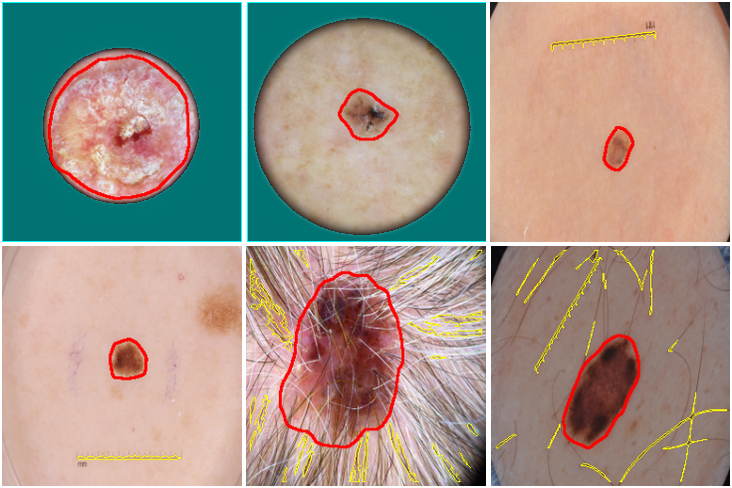
\includegraphics[width=0.92\linewidth]{fig/artifact_masks.png}
\caption{Automatically generated masks on ISIC~2019 images (red: lesion). Top left and center: dark corners (shaded cyan); top right and bottom left: rulers and bottom center/right: hair, detected as thin dark structures (yellow). Artifact masks never overlap the lesion.}
\label{fig:masks}
\end{figure}

\subsection{How masks are used, and why they cannot leak}
Masks enter the pipeline at exactly three places: the training losses, the constrained projection, and the attribution metrics of the evaluation. The classifier itself never receives a mask: at test time it sees only the image, so the classification results do not depend on whether a test mask is correct. Leakage is prevented at every stage.
\begin{itemize}
\item \emph{Split first.} The train/validation/test split is computed from image identifiers, lesion identifiers and image content only, before any model, including the segmentation network, is trained.
\item \emph{Group-level split.} Images are grouped by lesion identifier and, in addition, by near-duplicate pairs, so that re-acquisitions and resized copies of the same lesion cannot end up in different sets (Section~\ref{sec:data}). An audit of the final split finds no shared group, no shared lesion identifier and no shared image between any two of the three sets, and all 342 near-identical pairs (thumbnail correlation $\geq0.97$) as well as all other verified near-duplicate pairs lie within a single set.
\item \emph{Training-only supervision.} The segmentation network is trained on the 8{,}163 training-split masks only; the 1{,}852 expert masks of the validation and test splits are used solely to measure its accuracy. The mask-based losses and the projection use training images only. Thresholds and checkpoints are chosen on the validation split, and the last-layer re-optimization uses training activations only.
\item \emph{Label-free masks.} Neither the segmentation network nor the artifact detectors see a diagnosis, so a mask cannot carry label information from one image to another.
\item \emph{Untouched external sets.} Derm7pt, PAD-UFES-20 and PH2 are used only for evaluation. External images flagged as possible near-duplicates of ISIC training images (8, 6 and 7 images) change no external AUC by more than 0.004 when they are removed.
\end{itemize}

\section{Experimental Setup}
\subsection{Data and leakage-free split}
\label{sec:data}
The task is melanoma versus all other diagnoses on the 25{,}331 training images of ISIC~2019 (HAM10000~\cite{tschandl2018}, BCN20000~\cite{combalia2019} and MSK~\cite{codella2018}), of which 4{,}522 (17.9\%) are melanomas. All images are resized to $256\times256$. Unlike common practice, we keep the 2{,}084 MSK images that lack a lesion identifier. To avoid leakage we group images not only by lesion identifier but also by near-duplicate pairs (perceptual-hash distance $\leq8$ and a thumbnail correlation of at least 0.9 for both the full and the central image). Grouping look-alike pairs errs on the safe side, since it can only remove leakage. The 13{,}259 resulting groups are split into ten stratified folds, one for testing and one for validation (Table~\ref{tab:data}). Table~\ref{tab:dist} shows that the diagnoses, the three sources, the two kinds of lesion mask and the four artifact types are distributed almost identically over the three sets, so differences between validation and test results cannot be explained by a shift in composition. No group and no lesion identifier is shared between sets. As external test sets we use Derm7pt~\cite{kawahara2019}, which provides a dermoscopic and a clinical image for each of its 1{,}011 cases (melanomas include \emph{in situ} lesions and metastases), and the smartphone images of PAD-UFES-20~\cite{pacheco2020}. PH2 serves only to check the segmentation, because the copy available to us has no diagnoses. None of the external images is used for training or for choosing thresholds or models.

\begin{table}[t]
\caption{Data (number of images). Thresholds and checkpoints are selected on ISIC validation; all other sets are used for testing only.}
\label{tab:data}
\centering
\setlength{\tabcolsep}{5pt}
\begin{tabular}{lrrrr}
\toprule
Set & Benign & Melanoma & Total & Mel.\,\% \\
\midrule
ISIC 2019 train & 16{,}895 & 3{,}657 & 20{,}552 & 17.8 \\
ISIC 2019 validation & 1{,}984 & 475 & 2{,}459 & 19.3 \\
ISIC 2019 test & 1{,}930 & 390 & 2{,}320 & 16.8 \\
ISIC 2019 total, of which & 20{,}809 & 4{,}522 & 25{,}331 & 17.9 \\
\quad source BCN20000 & 9{,}556 & 2{,}857 & 12{,}413 & 23.0 \\
\quad source HAM10000 & 8{,}902 & 1{,}113 & 10{,}015 & 11.1 \\
\quad source MSK & 2{,}351 & 552 & 2{,}903 & 19.0 \\
\midrule
Derm7pt, dermoscopic & 759 & 252 & 1{,}011 & 24.9 \\
Derm7pt, clinical & 759 & 252 & 1{,}011 & 24.9 \\
PAD-UFES-20 & 2{,}246 & 52 & 2{,}298 & 2.3 \\
PH2 (segmentation only) & -- & -- & 200 & -- \\
\bottomrule
\multicolumn{5}{l}{\footnotesize Each source is split about 81/10/9\% into train/validation/test.}
\end{tabular}
\end{table}

\begin{table}[t]
\caption{Distribution of the ISIC~2019 split: diagnoses, acquisition sources (images / melanomas), provenance of the lesion masks and prevalence of the detected artifacts. All proportions are nearly identical across the three sets.}
\label{tab:dist}
\centering
\footnotesize
\setlength{\tabcolsep}{2.5pt}
\begin{tabular}{lrrrr}
\toprule
& Train & Val. & Test & All \\
\midrule
\multicolumn{5}{l}{\emph{Diagnosis}} \\
Melanoma & 3{,}657 & 475 & 390 & 4{,}522 \\
Nevus & 10{,}523 & 1{,}208 & 1{,}144 & 12{,}875 \\
Basal cell carc. & 2{,}671 & 322 & 330 & 3{,}323 \\
Actinic keratosis & 693 & 80 & 94 & 867 \\
Benign keratosis & 2{,}095 & 278 & 251 & 2{,}624 \\
Dermatofibroma & 193 & 16 & 30 & 239 \\
Vascular lesion & 201 & 27 & 25 & 253 \\
Squamous cell carc. & 519 & 53 & 56 & 628 \\
\midrule
\multicolumn{5}{l}{\emph{Source (images / melanomas)}} \\
BCN20000 & 10{,}037/2{,}299 & 1{,}225/310 & 1{,}151/248 & 12{,}413/2{,}857 \\
HAM10000 & 8{,}163/917 & 952/103 & 900/93 & 10{,}015/1{,}113 \\
MSK & 2{,}352/441 & 282/62 & 269/49 & 2{,}903/552 \\
\midrule
\multicolumn{5}{l}{\emph{Lesion mask}} \\
Expert (HAM10000) & 8{,}163 & 952 & 900 & 10{,}015 \\
Predicted (BCN, MSK) & 12{,}389 & 1{,}507 & 1{,}420 & 15{,}316 \\
Valid mask (\%) & 99.91 & 99.96 & 100.0 & -- \\
\midrule
\multicolumn{5}{l}{\emph{Artifact prevalence (\%)}} \\
Dark corners & 25.5 & 25.7 & 25.1 & -- \\
Thin dark structures & 24.2 & 25.7 & 23.4 & -- \\
Bright structures & 13.8 & 14.4 & 13.3 & -- \\
Ink / patches & 1.6 & 1.9 & 2.0 & -- \\
\bottomrule
\end{tabular}
\end{table}

\subsection{Models and training}
The eight configurations differ only in the components listed below; backbone (ImageNet-pretrained DenseNet-121), input size ($224\times224$), data, split and schedule are the same. \textbf{CNN}: backbone, global average pooling and a linear layer (black box). \textbf{PPN-std}: ProtoPNet with standard augmentation (random crop, horizontal flip). \textbf{PPN}: ProtoPNet with strong augmentation (random resized crop, scale $[0.4,1]$; horizontal and vertical flips; $\pm20\%$ brightness, contrast, saturation), used by all following models. \textbf{PPN-FA}: PPN with the IAIA-BL fine-annotation loss~\cite{barnett2021} on our lesion masks ($\lambda=10^{-3}$). \textbf{Ours}: lesion attraction and constrained projection; in the main runs the objective also contains the exploratory term $\Lart$, i.e.\ Eq.~(\ref{eq:loss}) with $\lambda_l=\lambda_a=1$. \textbf{Ablations}: without $\Lles$ (Ours-noLes), without $\Lart$ (Ours-noArt, i.e.\ the two core components only), and with the standard projection (Ours-stdPush).

We train with Adam, a batch size of 64 and mixed precision. The first 5 epochs keep the backbone frozen and train the add-on layers and prototypes at a learning rate of $3\times10^{-3}$. The next 15 epochs train all layers (backbone $10^{-4}$, weight decay $10^{-3}$, learning rate divided by 10 every 5 epochs). The projection and 5 last-layer epochs follow; the CNN is trained for the same 20 epochs. Class weights are 0.608 and 2.81. For the CNN we keep the checkpoint with the best validation AUC, whereas prototype models are always evaluated after the projection. Each configuration is run with seeds 0, 1 and 2, which takes about 30 minutes per run on an NVIDIA T4.

\subsection{Evaluation protocol}
\textbf{Classification.} The threshold of each run is fixed on the ISIC validation set with the Youden index and then reused for every test set. AUC, balanced accuracy (BAcc), sensitivity and specificity are given as mean $\pm$ std over the seeds. For significance testing we average the probabilities of the three seeds (seed ensemble), compute 95\% confidence intervals from 1{,}000 bootstrap resamples (resampling lesion groups on ISIC) and compare AUCs with the paired DeLong test~\cite{delong1988,sun2014}.

\textbf{Attribution.} For a prototype model we take the three most activated prototypes, upsample their similarity maps to $224\times224$ and keep the top 5\% of pixels, i.e.\ the 95th-percentile region that ProtoPNet uses for visualization. For the CNN we use the class-activation map; with a global-average-pooling head it coincides with Grad-CAM~\cite{selvaraju2017} up to a positive factor~\cite{zhou2016}. From this hot region we compute the share that lies on the lesion and on artifacts, check whether its maximum falls on an artifact (pointing), and compute the \emph{enrichment}, the artifact share divided by the artifact area. An enrichment above 1 means that artifacts get more attention than their size alone would explain.

\textbf{Counterfactuals.} Each test image is modified in four ways, always outside a 4-pixel margin around the lesion: we draw a ruler along one border, 12--30 curved hairs, a dark vignette, or 2--4 purple ink arcs. In the opposite direction, we erase the thin dark structures found by the detector (real hair and ruler marks, 544 images) with Telea inpainting~\cite{telea2004}. As a null control, a region of the same shape is shifted onto artifact-free skin and inpainted as well. A check after every modification confirms that each lesion pixel is bit-identical to the original. We then record the mean $|\Delta p|$ of the melanoma probability and the rate of flipped decisions. For the three prototypes most active on the original image we also measure how much the explanation moves: the Spearman correlation $\rho$ of the top-1 map, the IoU of the hot regions and the \emph{capture}, the part of the new hot region that lies on inserted pixels. Seed-averaged per-image values are compared with the Wilcoxon signed-rank test.

\section{Results}
\subsection{Artifacts are associated with melanoma}
In the training split, melanomas show dark corners and bright structures significantly more often than other lesions (Table~\ref{tab:bias}). This could simply reflect the source of the images, since dark corners appear in 47\% of the BCN images but in only 5\% of the HAM images, and BCN also has the highest melanoma rate. Stratifying by source does not remove the effect, however. The Mantel--Haenszel odds ratios remain clearly above 1, and for dark corners the odds ratio exceeds 1 in each source separately (BCN 1.41, HAM 3.10, MSK 2.24). For thin dark structures and ink we find no association.

\begin{table}[t]
\caption{Artifact--melanoma association (training split). OR: odds ratio; MH: Mantel--Haenszel OR stratified by source.}
\label{tab:bias}
\centering
\setlength{\tabcolsep}{2.2pt}
\begin{tabular}{lccccc}
\toprule
Artifact & Prev. & $P(\mathrm{m}|\mathrm{a})$ & $P(\mathrm{m}|\neg\mathrm{a})$ & OR & MH OR [95\% CI] \\
\midrule
Dark corners & 25.5\% & .263 & .149 & 2.03 & 1.56 [1.43, 1.69] \\
Bright structures & 13.8\% & .266 & .164 & 1.85 & 1.75 [1.59, 1.92] \\
Thin dark struct. & 24.2\% & .174 & .179 & 0.97 & 0.99 [0.90, 1.08] \\
Ink / patches & 1.6\% & .202 & .178 & 1.18 & 1.11 [0.85, 1.46] \\
Any & 48.8\% & .210 & .148 & 1.53 & 1.27 [1.17, 1.36] \\
\bottomrule
\end{tabular}
\end{table}

\begin{table*}[t]
\caption{Classification (mean $\pm$ std over 3 seeds; threshold from ISIC validation). Ens.: seed-ensemble AUC with 95\% bootstrap CI; $p$: paired DeLong test of the ensemble against Ours on ISIC test. Bold: best prototype model.}
\label{tab:cls}
\centering
\setlength{\tabcolsep}{3.4pt}
\begin{tabular}{lcccccccccc}
\toprule
& \multicolumn{6}{c}{ISIC 2019 test ($n=2{,}320$)} & \multicolumn{3}{c}{External AUC} \\
\cmidrule(lr){2-7}\cmidrule(lr){8-10}
Model & AUC & BAcc & Sens. & Spec. & Ens.\ AUC [95\% CI] & $p$ & Derm7pt-derm & Derm7pt-clin & PAD-UFES-20 \\
\midrule
CNN (black box) & .902$\pm$.006 & .814$\pm$.011 & .808$\pm$.044 & .820$\pm$.040 & .912 [.884, .935] & 3e-5 & .799$\pm$.023 & .704$\pm$.022 & .721$\pm$.022 \\
\midrule
PPN-std & .835$\pm$.013 & .752$\pm$.014 & .769$\pm$.063 & .734$\pm$.040 & .861 [.827, .888] & 6e-6 & .677$\pm$.027 & .624$\pm$.023 & .587$\pm$.019 \\
PPN & .825$\pm$.040 & .758$\pm$.010 & .786$\pm$.068 & .730$\pm$.087 & .866 [.830, .894] & 7e-4 & .688$\pm$.072 & .618$\pm$.038 & .665$\pm$.016 \\
PPN-FA (IAIA-BL) & .844$\pm$.008 & .744$\pm$.021 & .689$\pm$.045 & .800$\pm$.005 & .866 [.830, .895] & 4e-4 & .696$\pm$.024 & .640$\pm$.013 & .630$\pm$.059 \\
\textbf{Ours} & \textbf{.865$\pm$.006} & \textbf{.780$\pm$.014} & .734$\pm$.075 & \textbf{.825$\pm$.046} & \textbf{.884 [.850, .910]} & -- & \textbf{.749$\pm$.009} & \textbf{.657$\pm$.019} & .647$\pm$.108 \\
\midrule
Ours-noLes & .830$\pm$.015 & .746$\pm$.030 & .766$\pm$.091 & .726$\pm$.032 & .856 [.821, .885] & 8e-8 & .717$\pm$.016 & .636$\pm$.033 & .628$\pm$.047 \\
Ours-noArt & .859$\pm$.011 & .772$\pm$.003 & .733$\pm$.056 & .811$\pm$.054 & .877 [.845, .904] & .085 & .752$\pm$.014 & .637$\pm$.030 & .678$\pm$.018 \\
Ours-stdPush & .863$\pm$.005 & .785$\pm$.002 & .823$\pm$.043 & .747$\pm$.047 & .884 [.852, .911] & .85 & .747$\pm$.005 & .670$\pm$.019 & .658$\pm$.108 \\
\bottomrule
\end{tabular}
\end{table*}

\subsection{Classification}
On the ISIC test set, Ours reaches the highest AUC among the prototype models ($0.865\pm0.006$, ensemble $0.884$; Table~\ref{tab:cls}). The difference to PPN, PPN-std and PPN-FA is significant (DeLong $p\leq7\times10^{-4}$), and the results vary less between seeds (std 0.006 compared with 0.040 for PPN). The black-box CNN is still more accurate (ensemble 0.912), so interpretability keeps a price of about 3 AUC points; for PPN the gap is 4.6. The ranking does not depend on the last-layer re-optimization (Table~\ref{tab:ll}): with the five-epoch last layer of the training schedule the test AUCs of all prototype models are lower, but Ours remains the best (0.846 vs.\ 0.770 for PPN), and its AUC changes least (by 0.019 vs.\ 0.038--0.079 for the prototype baselines), which indicates that lesion-anchored prototypes keep their discriminative power after projection.

\begin{table}[t]
\caption{Effect of the last layer on ISIC test AUC (mean $\pm$ std over seeds). 5 ep.: last layer trained for the five epochs of the schedule; converged: re-optimized to convergence on training activations (used in all other tables).}
\label{tab:ll}
\centering
\setlength{\tabcolsep}{6pt}
\begin{tabular}{lcc}
\toprule
Model & 5 ep. & converged \\
\midrule
PPN-std & .797$\pm$.027 & .835$\pm$.013 \\
PPN & .770$\pm$.027 & .825$\pm$.040 \\
PPN-FA & .765$\pm$.023 & .844$\pm$.008 \\
\textbf{Ours} & \textbf{.846$\pm$.007} & \textbf{.865$\pm$.006} \\
Ours-noLes & .787$\pm$.045 & .830$\pm$.015 \\
Ours-noArt & .834$\pm$.029 & .859$\pm$.011 \\
Ours-stdPush & .841$\pm$.002 & .863$\pm$.005 \\
\bottomrule
\end{tabular}
\end{table} Externally, Ours has the highest prototype-model AUC on Derm7pt-dermoscopic (0.749; ensemble $p=1.7\times10^{-5}$ vs.\ PPN-FA, $2.8\times10^{-6}$ vs.\ PPN-std, $0.20$ vs.\ PPN, whose seed variance is high) and Derm7pt-clinical (0.657; $p=0.046$ vs.\ PPN). PAD-UFES-20 contains only 52 melanomas, and there none of the prototype models differs significantly from Ours. Excluding the external images flagged as possible ISIC near-duplicates (8, 6 and 7) changes each external AUC by at most 0.004.

\begin{table}[t]
\caption{Where the models look (ISIC test, mean $\pm$ std over seeds). Art.: hot-region fraction on artifacts in images with artifacts; Enr.: artifact enrichment; Point: maximum on an artifact; L-pr.: prototypes projected onto lesion cells (of 20).}
\label{tab:attr}
\centering
\setlength{\tabcolsep}{2.3pt}
\begin{tabular}{lccccc}
\toprule
Model & Lesion$\uparrow$ & Art.$\downarrow$ & Enr.$\downarrow$ & Point$\downarrow$ & L-pr. \\
\midrule
CNN & .466$\pm$.040 & .231$\pm$.024 & 1.52$\pm$.46 & .117$\pm$.007 & -- \\
PPN-std & .518$\pm$.036 & .082$\pm$.049 & 0.54$\pm$.31 & .050$\pm$.029 & 12.0 \\
PPN & .562$\pm$.012 & .066$\pm$.045 & 0.46$\pm$.04 & .042$\pm$.040 & 14.3 \\
PPN-FA & .530$\pm$.051 & .102$\pm$.024 & 0.68$\pm$.05 & .050$\pm$.006 & 10.0 \\
\textbf{Ours} & \textbf{.589$\pm$.040} & \textbf{.048$\pm$.015} & \textbf{0.37$\pm$.13} & \textbf{.013$\pm$.005} & \textbf{20.0} \\
\midrule
Ours-noLes & .565$\pm$.051 & .106$\pm$.056 & 0.67$\pm$.11 & .053$\pm$.029 & 20.0 \\
Ours-noArt & .594$\pm$.028 & .042$\pm$.008 & 0.40$\pm$.03 & .018$\pm$.007 & 20.0 \\
Ours-stdPush & .515$\pm$.063 & .086$\pm$.052 & 0.58$\pm$.30 & .034$\pm$.024 & 7.7 \\
\bottomrule
\end{tabular}
\end{table}

\begin{figure}[t]
\centering
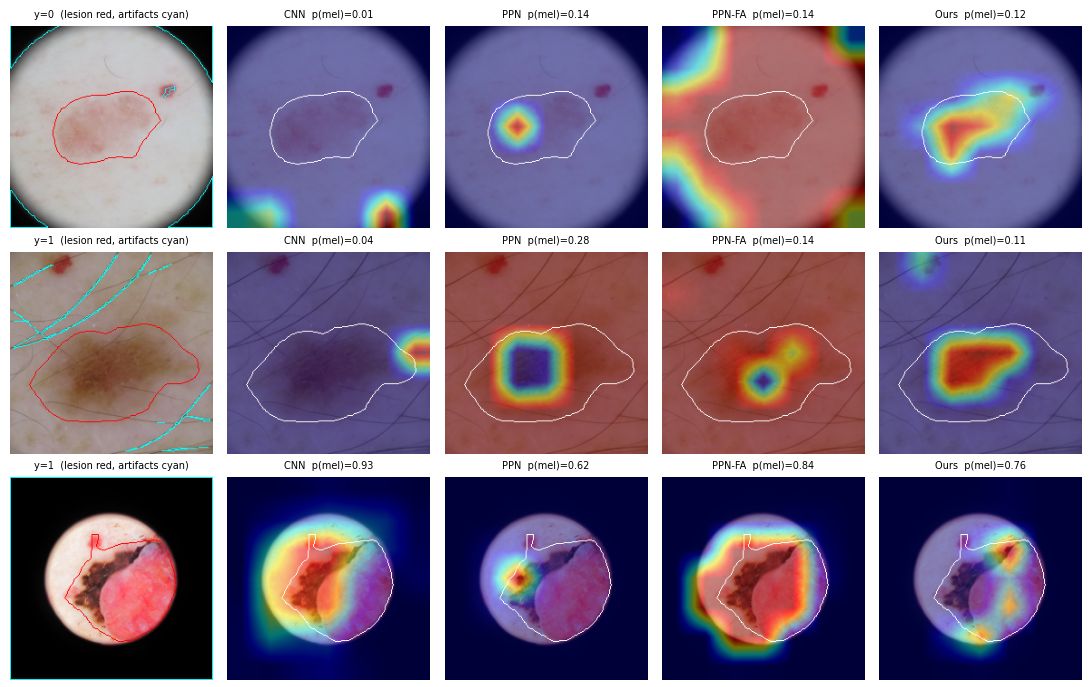
\includegraphics[width=0.92\linewidth]{fig/explanations_3rows.png}
\caption{ISIC test images with artifacts (left: lesion red, detected artifacts cyan). CNN: class-activation map; prototype models: map of the most activated prototype; $p$: melanoma probability (seed-0 models). Here the CNN and PPN-FA respond to dark corners and borders, whereas the top prototype of Ours stays on the lesion.}
\label{fig:expl}
\end{figure}

\subsection{Where the models look}
The black-box CNN is the model most drawn to artifacts (Table~\ref{tab:attr}, Fig.~\ref{fig:expl}). In images that contain artifacts, 23.1\% of its hot region lies on them (36.5\% when dark corners are present), 1.5 times more than their area would suggest, and in 11.7\% of the test images its maximum sits on an artifact. The prototype models look at artifacts less than their area would suggest, and Ours does so least: 4.8\% of the hot region (PPN 6.6\%, PPN-FA 10.2\%), an artifact maximum in 1.3\% of images (PPN 4.2\%), and the largest lesion fraction (58.9\%). All 20 prototypes of every Ours run are lesion patches, whereas PPN-FA projects on average 10.0 prototypes onto lesion and 2.0 onto artifact cells (Fig.~\ref{fig:protos}). Table~\ref{tab:attr2} breaks the artifact share down by type. Dark corners attract most of the attention that falls on artifacts: 36.5\% of the CNN hot region in images with dark corners, 9.8\% for PPN, 15.8\% for PPN-FA and 6.7\% for Ours. Thin dark structures and bright structures are small and receive at most 2\% from any model, and on ink Ours (3.2\%) stays below all prototype baselines (3.6--5.6\%). On the external Derm7pt-dermoscopic set the artifact pointing rate is again lowest for Ours (1.5\% vs.\ 4.4\% for PPN and 15.3\% for the CNN), as is the enrichment, although PPN places a larger hot-region fraction on the lesion there (0.79 vs.\ 0.73).

\begin{table}[t]
\caption{Attribution by artifact type (ISIC test; hot-region share on the given artifact in images that contain it) and on the external Derm7pt-dermoscopic set (mean over 3 seeds).}
\label{tab:attr2}
\centering
\setlength{\tabcolsep}{2.4pt}
\begin{tabular}{lcccc|ccc}
\toprule
& \multicolumn{4}{c|}{ISIC test, by type} & \multicolumn{3}{c}{Derm7pt-derm} \\
Model & DC & TS & SP & INK & Lesion & Point & Enr. \\
\midrule
CNN & .365 & .016 & .017 & .029 & .605 & .153 & .63 \\
PPN-std & .123 & .010 & .015 & .049 & .749 & .075 & .25 \\
PPN & .098 & .010 & .012 & .036 & .789 & .044 & .24 \\
PPN-FA & .158 & .010 & .010 & .056 & .760 & .077 & .28 \\
\textbf{Ours} & .067 & .011 & .016 & .032 & .734 & \textbf{.015} & \textbf{.18} \\
\midrule
Ours-noLes & .162 & .011 & .013 & .044 & .772 & .057 & .30 \\
Ours-noArt & .056 & .012 & .020 & .040 & .713 & .017 & .23 \\
Ours-stdPush & .129 & .012 & .019 & .030 & .633 & .033 & .35 \\
\bottomrule
\end{tabular}
\end{table}

\begin{figure*}[t]
\centering
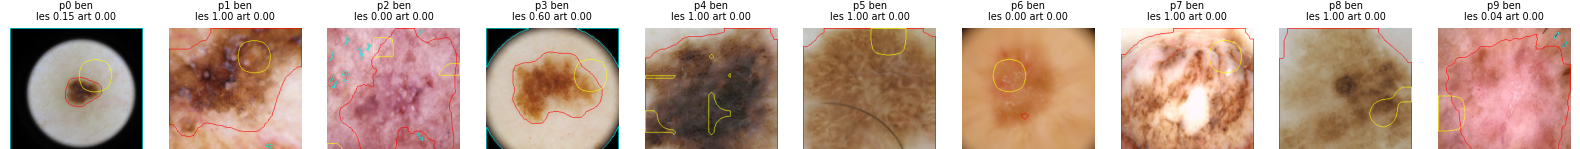
\includegraphics[width=\textwidth]{fig/prototypes_PPN_s0_ben.png}\\[1pt]
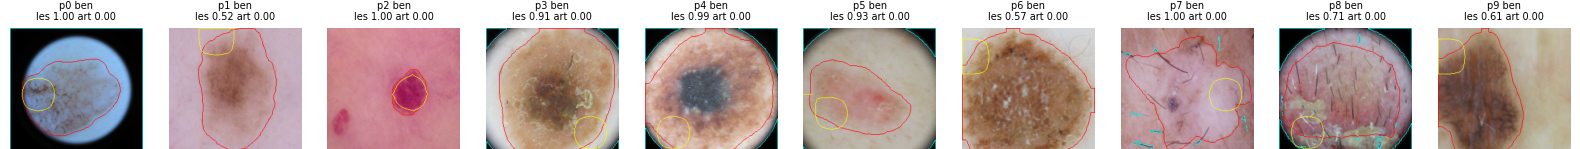
\includegraphics[width=\textwidth]{fig/prototypes_Ours_s0_ben.png}
\caption{Source patches of the ten benign-class prototypes of PPN (top) and Ours (bottom), seed 0 (``les''/``art'': lesion and artifact fraction of the projected cell; red: lesion; cyan: artifacts; yellow: 95th-percentile region of the prototype on its own source image). Four PPN prototypes come from background skin (lesion fraction 0.00--0.15); all prototypes of Ours lie on lesion tissue.}
\label{fig:protos}
\end{figure*}

\begin{table*}[t]
\caption{Counterfactual interventions on ISIC test (lesion pixels unchanged; mean over 3 seeds). Flip: decision changes (\%); $|\Delta p|$: mean absolute change of the melanoma probability; $\rho$: Spearman correlation of the top-1 prototype map before/after; Cap.: share of the new hot region on inserted pixels (\%).}
\label{tab:cf}
\centering
\setlength{\tabcolsep}{3.1pt}
\begin{tabular}{l cc cc cc cc cc cc cc cc}
\toprule
& \multicolumn{2}{c}{+Dark corners} & \multicolumn{2}{c}{+Ruler} & \multicolumn{2}{c}{+Hair} & \multicolumn{2}{c}{+Ink} & \multicolumn{2}{c}{Remove hair/ruler} & \multicolumn{2}{c}{Null control} & \multicolumn{2}{c}{Expl.: dark corners} & \multicolumn{2}{c}{Expl.: ruler} \\
\cmidrule(lr){2-3}\cmidrule(lr){4-5}\cmidrule(lr){6-7}\cmidrule(lr){8-9}\cmidrule(lr){10-11}\cmidrule(lr){12-13}\cmidrule(lr){14-15}\cmidrule(lr){16-17}
Model & Flip & $|\Delta p|$ & Flip & $|\Delta p|$ & Flip & $|\Delta p|$ & Flip & $|\Delta p|$ & Flip & $|\Delta p|$ & Flip & $|\Delta p|$ & $\rho\uparrow$ & Cap.$\downarrow$ & $\rho\uparrow$ & Cap.$\downarrow$ \\
\midrule
CNN & 6.1 & .049 & 5.6 & .049 & 12.5 & .104 & 9.8 & .080 & 4.7 & .036 & 1.0 & .008 & -- & -- & -- & -- \\
PPN-std & 10.9 & .060 & 8.3 & .041 & 14.9 & .092 & 9.9 & .058 & 8.8 & .036 & 4.3 & .013 & .635 & 7.1 & .773 & 1.5 \\
PPN & 10.9 & .067 & 7.5 & .045 & 14.0 & .096 & 9.5 & .062 & 7.4 & .045 & 3.6 & .019 & .680 & 6.1 & .804 & 1.1 \\
PPN-FA & 10.6 & .049 & 6.5 & .028 & 15.1 & .084 & 9.1 & .046 & 7.2 & .030 & 3.2 & .010 & .714 & 11.4 & .874 & 1.1 \\
\textbf{Ours} & \textbf{5.2} & \textbf{.035} & \textbf{3.6} & \textbf{.025} & \textbf{9.2} & \textbf{.081} & \textbf{5.6} & \textbf{.045} & \textbf{4.4} & .032 & 1.6 & .011 & \textbf{.918} & \textbf{3.4} & \textbf{.952} & \textbf{0.7} \\
\midrule
Ours-noLes & 10.2 & .053 & 8.7 & .040 & 14.3 & .083 & 10.1 & .049 & 8.3 & .042 & 3.9 & .016 & .705 & 8.6 & .827 & 1.7 \\
Ours-noArt & 5.4 & .036 & 3.5 & .023 & 8.7 & .061 & 6.1 & .041 & 4.4 & .027 & 1.0 & .011 & .884 & 3.4 & .949 & 1.0 \\
Ours-stdPush & 4.5 & .034 & 4.1 & .028 & 9.6 & .077 & 5.8 & .045 & 4.5 & .033 & 1.9 & .011 & .923 & 7.5 & .944 & 1.4 \\
\bottomrule
\end{tabular}
\end{table*}

\subsection{Counterfactual robustness}
Table~\ref{tab:cf} summarizes the interventions; in all 2{,}063--2{,}318 modified images per insertion type the lesion pixels were confirmed to be unchanged. Adding dark corners \emph{increases} the melanoma probability of every model (mean signed change $+0.041$ CNN, $+0.048$ PPN, $+0.020$ Ours), which matches the sign of the association in Table~\ref{tab:bias}. The models have absorbed the shortcut, and Ours has absorbed it least. Ours roughly halves the flip rate of PPN for dark corners (10.9\%$\rightarrow$5.2\%) and rulers (7.5\%$\rightarrow$3.6\%), reduces it for ink (9.5\%$\rightarrow$5.6\%) and hair (14.0\%$\rightarrow$9.2\%), and flips fewer decisions than the CNN for all four insertions. All per-image $|\Delta p|$ differences between Ours and PPN are significant (Wilcoxon $p<10^{-39}$), as are those against the CNN ($p\leq0.018$). Removing real hair and ruler marks changes more decisions than the null control for every model (Ours 4.4\% vs.\ 1.6\%), so the measured sensitivity stems from the artifacts, not from inpainting.

Its explanations also move the least (Fig.~\ref{fig:cf}). After adding dark corners its top-1 prototype map keeps $\rho=0.92$ (PPN 0.68), and only 3.4\% of its hot region moves onto the inserted pixels (PPN 6.1\%, PPN-FA 11.4\%; $p<10^{-100}$). The exception is ink: the arcs lie just outside the lesion border, where lesion-anchored prototypes respond, so 1.8\% of the hot region of Ours falls on ink vs.\ 1.0\% for PPN, although Ours still flips fewer decisions.

\begin{figure}[t]
\centering
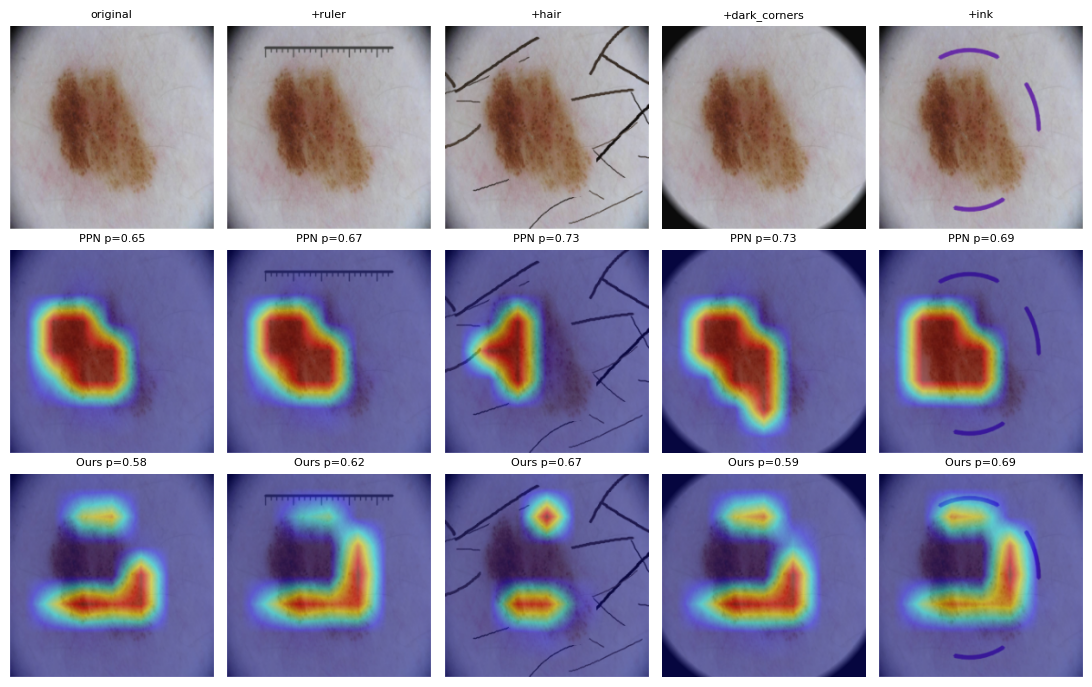
\includegraphics[width=0.92\linewidth]{fig/counterfactual_example_0.png}
\caption{Counterfactual example with unchanged lesion pixels. Rows 2--3: map of the prototype most active on the original image and melanoma probability $p$ for PPN and Ours.}
\label{fig:cf}
\end{figure}

\subsection{Ablation of the two core components}
\textbf{Lesion attraction} is the term behind the accuracy gain. Without it (Ours-noLes) the test AUC falls to 0.830 (DeLong $p=8\times10^{-8}$), the artifact share of the hot region more than doubles (4.8\%$\rightarrow$10.6\%), and the flip rates for dark corners, rulers and ink roughly double (Tables~\ref{tab:cls}--\ref{tab:cf}). Ours-noLes still uses the constrained projection, so all of its prototypes are lesion patches; the comparison therefore shows that a correct projection alone is not enough, the attention during training has to be anchored as well.

\textbf{The constrained projection} leaves the accuracy unchanged (Ours-stdPush, $p=0.85$) but determines what the prototypes \emph{are}: with the standard projection only 7.7 of 20 prototypes lie on the lesion, the artifact share of the hot region rises from 4.8\% to 8.6\%, and the share captured by added dark corners from 3.4\% to 7.5\% ($p<10^{-200}$). Accuracy alone would have hidden this difference, which is why we evaluate explanations directly.

\subsection{Negative result: artifact suppression}
\label{sec:lart}
We also explored a term that penalizes attention on artifacts directly. With $A_{ij}=\sum_{h,w}\alpha_{ij}M^A_i$, the attention mass of prototype $j$ on the artifacts of image $i$,
\begin{equation}
\Lart=\frac{1}{|\mathcal{B}|}\sum_{i\in\mathcal{B}}\sum_{j=1}^{m}\omega_{ij}A_{ij}.
\end{equation}
Removing it (Ours-noArt) degrades no metric. The AUC difference to Ours is not significant ($p=0.085$), the attribution scores are equivalent (artifact share 4.2\% vs.\ 4.8\%), and the counterfactual robustness is similar or even slightly better (e.g., $|\Delta p|$ 0.061 vs.\ 0.081 for added hair). We see two reasons. First, $\Lles$ already acts on a normalized attention, so increasing the lesion mass reduces the mass on artifacts automatically. Second, the constrained projection removes the remaining route by which an artifact could become part of a prototype. Since $\Lart$ is redundant, we do not count it as part of the method; the two core components (Ours-noArt) are the configuration we recommend, and Ours in the tables differs from it only by this term.

\subsection{Robustness to mask quality}
\label{sec:maskrob}
Predicted masks could, in principle, bias the results in two ways: a model could look ``on the lesion'' only by the measure of an imperfect mask, or the gains could appear only on the sources whose masks were predicted. We test both on the ISIC test set by splitting it by mask provenance into the 900 HAM10000 images with expert masks and the 1{,}420 BCN20000 and MSK images with predicted masks, and by repeating the attribution with lesion masks eroded or dilated by 5~pixels (Table~\ref{tab:maskrob}).

\begin{table*}[t]
\caption{Robustness to mask quality (ISIC test, mean $\pm$ std over 3 seeds). Left: attribution measured separately on images with expert masks (HAM10000, $n=900$) and with predicted masks (BCN20000 and MSK, $n=1{,}420$); Lesion, Art.\ and Point as in Table~\ref{tab:attr}. Middle: lesion fraction of the hot region when every lesion mask is eroded ($-5$\,px) or dilated ($+5$\,px). Right: test AUC per acquisition source (the classifier receives no mask at test time; $n$/melanomas: BCN 1{,}151/248, HAM 900/93, MSK 269/49).}
\label{tab:maskrob}
\centering
\setlength{\tabcolsep}{2.6pt}
\begin{tabular}{l|ccc|ccc|cc|ccc}
\toprule
& \multicolumn{3}{c|}{Expert masks (HAM10000)} & \multicolumn{3}{c|}{Predicted masks (BCN, MSK)} & \multicolumn{2}{c|}{Lesion, perturbed mask} & \multicolumn{3}{c}{AUC by source} \\
Model & Lesion$\uparrow$ & Art.$\downarrow$ & Point$\downarrow$ & Lesion$\uparrow$ & Art.$\downarrow$ & Point$\downarrow$ & $-5$\,px & $+5$\,px & BCN & HAM & MSK \\
\midrule
CNN & .444$\pm$.044 & .043$\pm$.014 & .015$\pm$.006 & .480$\pm$.038 & .277$\pm$.026 & .182$\pm$.010 & .434$\pm$.038 & .496$\pm$.040 & .883$\pm$.012 & .934$\pm$.003 & .861$\pm$.002 \\
\midrule
PPN-std & .416$\pm$.085 & .016$\pm$.005 & .004$\pm$.002 & .582$\pm$.046 & .098$\pm$.059 & .079$\pm$.047 & .480$\pm$.036 & .552$\pm$.035 & .825$\pm$.018 & .880$\pm$.016 & .711$\pm$.022 \\
PPN & .446$\pm$.053 & .014$\pm$.001 & .005$\pm$.005 & \textbf{.635$\pm$.015} & .079$\pm$.056 & .065$\pm$.062 & .525$\pm$.013 & .595$\pm$.012 & .819$\pm$.051 & .860$\pm$.034 & .692$\pm$.016 \\
PPN-FA & .423$\pm$.045 & .019$\pm$.003 & .004$\pm$.002 & .599$\pm$.060 & .123$\pm$.030 & .080$\pm$.011 & .491$\pm$.055 & .567$\pm$.047 & .834$\pm$.009 & .896$\pm$.004 & .699$\pm$.014 \\
\textbf{Ours} & \textbf{.534$\pm$.062} & \textbf{.013$\pm$.005} & \textbf{.002$\pm$.001} & .624$\pm$.026 & \textbf{.056$\pm$.018} & \textbf{.021$\pm$.008} & \textbf{.534$\pm$.039} & \textbf{.640$\pm$.041} & \textbf{.852$\pm$.008} & \textbf{.906$\pm$.006} & \textbf{.761$\pm$.018} \\
\midrule
Ours-noLes & .503$\pm$.089 & .023$\pm$.013 & .007$\pm$.006 & .603$\pm$.064 & .126$\pm$.071 & .082$\pm$.049 & .525$\pm$.055 & .601$\pm$.047 & .815$\pm$.017 & .879$\pm$.013 & .704$\pm$.032 \\
Ours-noArt & .543$\pm$.030 & .013$\pm$.003 & .003$\pm$.001 & .626$\pm$.043 & .050$\pm$.010 & .028$\pm$.010 & .541$\pm$.041 & .644$\pm$.023 & .853$\pm$.013 & .893$\pm$.008 & .737$\pm$.023 \\
Ours-stdPush & .459$\pm$.043 & .018$\pm$.007 & .003$\pm$.001 & .550$\pm$.075 & .103$\pm$.063 & .054$\pm$.039 & .466$\pm$.060 & .561$\pm$.065 & .852$\pm$.009 & .904$\pm$.004 & .749$\pm$.005 \\
\bottomrule
\end{tabular}
\end{table*}

\textbf{Expert masks alone.} On the HAM10000 test images, where the attribution is measured against masks drawn by experts and not by our segmentation network, Ours places 53.4\% of its hot region on the lesion, against 41.6--44.6\% for the three prototype baselines and 44.4\% for the CNN. Its advantage in lesion focus is thus \emph{larger} on expert masks (+8.8 points over the best baseline) than on the whole test set (+2.7 points), so it is not produced by errors of the predicted masks. HAM10000 images contain few and small artifacts (dark corners in about 5\%), so all artifact scores are low on this subset; Ours still has the lowest artifact share (1.3\%) and pointing rate (0.2\%). On the images with predicted masks the artifact advantage is large: 5.6\% of the hot region of Ours lies on artifacts (PPN 7.9\%, PPN-FA 12.3\%, CNN 27.7\%), and its maximum falls on an artifact in 2.1\% of the images (PPN 6.5\%, CNN 18.2\%). Here PPN places a slightly larger fraction on the lesion (63.5\% vs.\ 62.4\%, within one standard deviation).

\textbf{Perturbed masks.} Eroding or dilating every lesion mask by 5~pixels at the $256\times256$ mask resolution shifts the lesion fractions of all models in the same direction. The order of the five main models is identical at $-5$, $0$ and $+5$~pixels (Ours $>$ PPN $>$ PPN-FA $>$ PPN-std $>$ CNN), although the margin of Ours over PPN shrinks to 0.9 points under erosion and grows to 4.5 points under dilation. Because the artifact masks are computed independently of the lesion masks, the artifact share and the pointing rate of every model change by at most 0.001 and the enrichment by at most 0.011.

\textbf{Classification per source.} The classifier receives no mask at test time, but its training used expert masks for HAM10000 and predicted masks for the other two sources. Ours is the most accurate prototype model in every source: on HAM10000, with expert training masks (0.906 vs.\ 0.896 for PPN-FA), and on BCN20000 (0.852 vs.\ 0.834) and MSK (0.761 vs.\ 0.711 for PPN-std), whose training masks were predicted. The gain is therefore not tied to one type of mask.

\begin{table}[t]
\caption{Counterfactual flip rate by mask provenance (ISIC test, mean over 3 seeds). Artifacts are inserted outside a 4-pixel margin around the lesion mask, so for the expert subset the protected region is exact.}
\label{tab:cfprov}
\centering
\setlength{\tabcolsep}{4.5pt}
\begin{tabular}{lcccc}
\toprule
& \multicolumn{2}{c}{+ Dark corners} & \multicolumn{2}{c}{+ Ruler} \\
\cmidrule(lr){2-3}\cmidrule(lr){4-5}
Model & Expert & Predicted & Expert & Predicted \\
\midrule
CNN & .071 & \textbf{.055} & .039 & .067 \\
PPN-std & .101 & .113 & .061 & .097 \\
PPN & .100 & .115 & .059 & .085 \\
PPN-FA & .103 & .107 & .047 & .077 \\
\textbf{Ours} & \textbf{.044} & .057 & \textbf{.023} & \textbf{.044} \\
\bottomrule
\end{tabular}
\end{table}

\textbf{Counterfactuals per provenance.} The counterfactual protocol uses the lesion mask to decide where artifacts may be drawn. If a predicted mask were too small, inserted artifacts could touch the true lesion and change the decision for the wrong reason. Table~\ref{tab:cfprov} shows that this is not what drives the results: on the expert-mask subset, where the protected region is exact, Ours flips the fewest decisions of all models for both insertions (dark corners 4.4\%, rulers 2.3\%), less than half of the prototype baselines. On the predicted-mask subset it flips the fewest decisions among the prototype models and as few as the CNN for dark corners (5.7\% vs.\ 5.5\%). The mean $|\Delta p|$ of Ours is also the smallest in both subsets (0.035--0.036 for dark corners vs.\ 0.043--0.068 for the other models).

In summary, the main conclusions (more lesion focus, less use of artifacts, fewer flipped decisions and higher accuracy than the prototype baselines) hold on the images with expert masks, under $\pm5$-pixel mask errors and in every acquisition source.

\section{Discussion and Limitations}
Tying prototype attention to the lesion made the prototype network both more accurate and more faithful, and restricting the projection ensures that its explanations are built from lesion tissue. The two components play different roles: lesion attraction changes what the network learns, whereas the constrained projection changes what it shows to the user. Neither role is visible in the AUC alone.

\textbf{Dependence on masks.} The approach needs lesion masks during training, and this is its main practical requirement. Three properties keep the dependence limited. First, the masks are needed only for training; deployment requires nothing but the image. Second, the masks are generated automatically from public expert segmentations of a single source (HAM10000), so no new annotation is needed for a new dataset of dermoscopic images. Third, the lesion-attraction term uses masks only through coarse $7\times7$ cell fractions and the projection only through a 50\% threshold, both of which tolerate boundary errors of a few pixels; Section~\ref{sec:maskrob} confirms that the conclusions hold on images with expert masks alone and under deliberate erosion or dilation of the masks.

\textbf{Limitations.} (i)~A gap of about 3 AUC points to the black-box CNN remains. (ii)~For BCN20000 and MSK no expert masks exist, so the predicted masks of these sources can only be validated indirectly (held-out HAM10000 images, PH2, and the subset analysis). The bright-structure detector also responds to light hairs, and other artifacts (e.g., gel borders) are not modeled. (iii)~Inserted artifacts are synthetic; we mitigated this with the removal of real artifacts and a null control. (iv)~The $7\times7$ latent grid limits the spatial resolution of the explanations. (v)~External gains are significant on Derm7pt but not on the small PAD-UFES-20 melanoma set, and a single backbone was studied, as required for a controlled comparison.

\section{Conclusion}
Standard and prototype classifiers trained on ISIC~2019 do exploit artifact shortcuts, and a prototype network can be anchored to the lesion without manual annotation. Two components suffice: lesion attraction on the prototype attention and a projection restricted to artifact-free lesion patches; an additional artifact-suppression term proved redundant. In our same-backbone, leakage-controlled comparison the lesion-anchored model was the most accurate prototype model, relied least on artifacts, and changed its decisions and explanations least when artifacts were inserted or removed around an unchanged lesion. Because the counterfactual protocol does not depend on the architecture, it can also be used to check the faithfulness of other interpretable classifiers.

\begin{thebibliography}{00}
\bibitem{esteva2017} A. Esteva \emph{et al.}, ``Dermatologist-level classification of skin cancer with deep neural networks,'' \emph{Nature}, vol.~542, no.~7639, pp.~115--118, 2017.
\bibitem{geirhos2020} R. Geirhos \emph{et al.}, ``Shortcut learning in deep neural networks,'' \emph{Nature Machine Intelligence}, vol.~2, pp.~665--673, 2020.
\bibitem{winkler2019} J. K. Winkler \emph{et al.}, ``Association between surgical skin markings in dermoscopic images and diagnostic performance of a deep learning convolutional neural network for melanoma recognition,'' \emph{JAMA Dermatology}, vol.~155, no.~10, pp.~1135--1141, 2019.
\bibitem{bissoto2019} A. Bissoto, M. Fornaciali, E. Valle, and S. Avila, ``(De)constructing bias on skin lesion datasets,'' in \emph{Proc. IEEE/CVF CVPR Workshops}, 2019.
\bibitem{bissoto2020} A. Bissoto, E. Valle, and S. Avila, ``Debiasing skin lesion datasets and models? Not so fast,'' in \emph{Proc. IEEE/CVF CVPR Workshops}, 2020.
\bibitem{bissoto2022} A. Bissoto, C. Barata, E. Valle, and S. Avila, ``Artifact-based domain generalization of skin lesion models,'' in \emph{Proc. ECCV Workshops}, 2022.
\bibitem{yan2023} S. Yan, C. Liu, Z. Yu, L. Ju, D. Mahapatra, V. Mar, M. Janda, P. Soyer, and Z. Ge, ``EPVT: Environment-aware prompt vision transformer for domain generalization in skin lesion recognition,'' in \emph{Proc. MICCAI}, 2023.
\bibitem{bevan2022} P. Bevan and A. Atapour-Abarghouei, ``Skin deep unlearning: Artefact and instrument debiasing in the context of melanoma classification,'' in \emph{Proc. Int. Conf. Machine Learning (ICML)}, 2022.
\bibitem{rudin2019} C. Rudin, ``Stop explaining black box machine learning models for high stakes decisions and use interpretable models instead,'' \emph{Nature Machine Intelligence}, vol.~1, pp.~206--215, 2019.
\bibitem{chen2019} C. Chen, O. Li, D. Tao, A. Barnett, C. Rudin, and J. K. Su, ``This looks like that: Deep learning for interpretable image recognition,'' in \emph{Advances in Neural Information Processing Systems (NeurIPS)}, vol.~32, 2019.
\bibitem{hoffmann2021} A. Hoffmann, C. Fanconi, R. Rade, and J. Kohler, ``This looks like that... does it? Shortcomings of latent space prototype interpretability in deep networks,'' in \emph{ICML Workshop on Theoretic Foundation, Criticism, and Application Trend of Explainable AI}, 2021.
\bibitem{barnett2021} A. J. Barnett \emph{et al.}, ``A case-based interpretable deep learning model for classification of mass lesions in digital mammography,'' \emph{Nature Machine Intelligence}, vol.~3, pp.~1061--1070, 2021.
\bibitem{bontempelli2023} A. Bontempelli, S. Teso, K. Tentori, F. Giunchiglia, and A. Passerini, ``Concept-level debugging of part-prototype networks,'' in \emph{Proc. Int. Conf. Learning Representations (ICLR)}, 2023.
\bibitem{ross2017} A. S. Ross, M. C. Hughes, and F. Doshi-Velez, ``Right for the right reasons: Training differentiable models by constraining their explanations,'' in \emph{Proc. IJCAI}, 2017, pp.~2662--2670.
\bibitem{rieger2020} L. Rieger, C. Singh, W. J. Murdoch, and B. Yu, ``Interpretations are useful: Penalizing explanations to align neural networks with prior knowledge,'' in \emph{Proc. Int. Conf. Machine Learning (ICML)}, 2020, pp.~8116--8126.
\bibitem{adebayo2018} J. Adebayo, J. Gilmer, M. Muelly, I. Goodfellow, M. Hardt, and B. Kim, ``Sanity checks for saliency maps,'' in \emph{Advances in Neural Information Processing Systems (NeurIPS)}, vol.~31, 2018.
\bibitem{huang2017} G. Huang, Z. Liu, L. van der Maaten, and K. Q. Weinberger, ``Densely connected convolutional networks,'' in \emph{Proc. IEEE CVPR}, 2017, pp.~4700--4708.
\bibitem{tschandl2018} P. Tschandl, C. Rosendahl, and H. Kittler, ``The HAM10000 dataset, a large collection of multi-source dermatoscopic images of common pigmented skin lesions,'' \emph{Scientific Data}, vol.~5, art.~180161, 2018.
\bibitem{combalia2019} M. Combalia \emph{et al.}, ``BCN20000: Dermoscopic lesions in the wild,'' arXiv:1908.02288, 2019.
\bibitem{codella2018} N. C. F. Codella \emph{et al.}, ``Skin lesion analysis toward melanoma detection: A challenge at the 2017 International Symposium on Biomedical Imaging (ISBI), hosted by the International Skin Imaging Collaboration (ISIC),'' in \emph{Proc. IEEE ISBI}, 2018, pp.~168--172.
\bibitem{chen2017deeplab} L.-C. Chen, G. Papandreou, F. Schroff, and H. Adam, ``Rethinking atrous convolution for semantic image segmentation,'' arXiv:1706.05587, 2017.
\bibitem{howard2019} A. Howard \emph{et al.}, ``Searching for MobileNetV3,'' in \emph{Proc. IEEE/CVF ICCV}, 2019, pp.~1314--1324.
\bibitem{mendonca2013} T. Mendon\c{c}a, P. M. Ferreira, J. S. Marques, A. R. S. Mar\c{c}al, and J. Rozeira, ``PH$^2$ -- A dermoscopic image database for research and benchmarking,'' in \emph{Proc. IEEE EMBC}, 2013, pp.~5437--5440.
\bibitem{lee1997} T. Lee, V. Ng, R. Gallagher, A. Coldman, and D. McLean, ``DullRazor: A software approach to hair removal from images,'' \emph{Computers in Biology and Medicine}, vol.~27, no.~6, pp.~533--543, 1997.
\bibitem{kawahara2019} J. Kawahara, S. Daneshvar, G. Argenziano, and G. Hamarneh, ``Seven-point checklist and skin lesion classification using multitask multimodal neural nets,'' \emph{IEEE J. Biomedical and Health Informatics}, vol.~23, no.~2, pp.~538--546, 2019.
\bibitem{pacheco2020} A. G. C. Pacheco \emph{et al.}, ``PAD-UFES-20: A skin lesion dataset composed of patient data and clinical images collected from smartphones,'' \emph{Data in Brief}, vol.~32, art.~106221, 2020.
\bibitem{delong1988} E. R. DeLong, D. M. DeLong, and D. L. Clarke-Pearson, ``Comparing the areas under two or more correlated receiver operating characteristic curves: A nonparametric approach,'' \emph{Biometrics}, vol.~44, no.~3, pp.~837--845, 1988.
\bibitem{sun2014} X. Sun and W. Xu, ``Fast implementation of DeLong's algorithm for comparing the areas under correlated receiver operating characteristic curves,'' \emph{IEEE Signal Processing Letters}, vol.~21, no.~11, pp.~1389--1393, 2014.
\bibitem{zhou2016} B. Zhou, A. Khosla, A. Lapedriza, A. Oliva, and A. Torralba, ``Learning deep features for discriminative localization,'' in \emph{Proc. IEEE CVPR}, 2016, pp.~2921--2929.
\bibitem{selvaraju2017} R. R. Selvaraju, M. Cogswell, A. Das, R. Vedantam, D. Parikh, and D. Batra, ``Grad-CAM: Visual explanations from deep networks via gradient-based localization,'' in \emph{Proc. IEEE ICCV}, 2017, pp.~618--626.
\bibitem{telea2004} A. Telea, ``An image inpainting technique based on the fast marching method,'' \emph{J. Graphics Tools}, vol.~9, no.~1, pp.~23--34, 2004.
\end{thebibliography}

\end{document}
